\documentclass[a4paper, 12pt]{article}
\usepackage[czech]{babel}
\usepackage[utf8]{inputenc}
\usepackage{graphicx}
\usepackage{float}
\usepackage[hang]{caption}
\usepackage[top=3cm, bottom=2cm, right=2.5cm, left=2.5cm]{geometry}
\usepackage{hyperref}
\usepackage{natbib}		
\usepackage{mathtools}
\usepackage{amsmath}
\bibpunct{(}{)}{;}{a}{,}{;}	

% --------<<< ------------------------- >>>--------

\begin{document}

\begin{center}
\textsc{Charles University} \\ 
\textsc{Faculty of Social Sciences}\\ 
\textsc{Institute of Economic Studies}\\[0.5em]
Data Processing in Python\\
SS 2022/2023\\ %[2em]
\end{center}

\begin{minipage}{1\textwidth}
\begin{center}
\title{\textbf{\emph{Project Report: 
Examination of Criminality in the Czech Republic based on Socio-Economic Determinants}}}
\author{\textbf{Tomáš Barhoň, Radim Plško}}
\date{August 2023}

\maketitle
\end{center}
\thispagestyle{empty}
\end{minipage}

\newpage %
\section{Introduction}
\paragraph{\normalfont{This report provides an overview of a project conducted by Tomáš Barhoň and Radim Plško for the Data Processing in Python class in the summer semester 2022/23. The project aims to study the impact of socio-economic indicators on the level of economic criminality in different regions of the Czech Republic ("obce s rozšířenou působností").}}

\section{Data Source}
\paragraph{\normalfont{The primary data source for this project is the https://kriminalita.policie.cz/ API, which provides information about various types of crimes and their precise geographical locations ("points of crimes"). Therefore, in order to be able to work with crimes on the level of regions ("ORP"), we needed to fit these points of crime to the geographical locations of ORPs.}}

\paragraph{\normalfont{The socio-economic data were obtained from various open-data sources, but mainly from PAQ research (https://www.datapaq.cz/) where all data were recorded on the level of ORP from the beginning which was the most convenient for us.}}

\paragraph{\normalfont{The study focused on the following four socio-economic indicators:}}

\begin{enumerate}
\item Lidé v exekuci (2021) - The percentage of people with foreclosure.
\item Podíl lidí bez středního vzdělání (2021) - The percentage of people without completed high school education.
\item Domácnosti čerpající přídavek na živobytí (2020) - The percentage of households receiving social benefits.
\item Propadání (průměr 2015–2021) - The percentage of children that obtain a grade of 5 from any subject at the end of the summer semester.
\end{enumerate}

\paragraph{\normalfont{In order to be able to conduct such analysis we made some assumptionts to our data. As there was not enough data for this specific granuality we had to take data from not exactly matching time periods. Our assumption is that the socio-economical variables that we have chosen are relatively stable over time thus we only tried to get the data from the correct period to some plausible extent.}}

\section{Crime Data}
\paragraph{\normalfont{The crime data was subset to meet specific conditions. The crimes included in the study are illegal, verifiable, and of an economic nature, such as thefts and burglaries - to be most relevant to the case of chosen specific socio-economic variables. The data was analyzed for the period from 2021 to June 2023, yielding about 500,000 criminal records. An import step in the analysis is that we did divide the ammounts in each ORP by its population as not ORPs do have the population which would leed to incorrect conclusions. It might be suggested that the data should be also for instance divided by the number of months in which it was analyzed but we did not make this choice at the time of our analysis as it does not affect our research. However, if anyone would like to compare it with different analysis this change would have to be considered.}}

\section{Code Overview}

\paragraph{\normalfont{In our code we utilized multiple visualization and data manipulation packages such as numpy, pandas, seaborn, matplotlib, folium, geopandas, pytest, shapely and two our modules visualizer, data API downloader.}}

\paragraph{\normalfont{We used jupyter notebookes for most of our visualizations as the final output of our project. However, we wanted to make them as clean as possible and wanted to help others with similar research ides. Thus we created two our own modules that do have classes which can do a lot of tasks useful even outside of our project. We used numpy style documentation to document them. Our main output is a set of geographical visualization which employ a combination of tabular data with geojson created from a geographical shapefile downloaded from the "ČZUK" website.}}

\paragraph{\normalfont{The main notebook where you can find all our analysis for this report is app/main.ipynb but there are 3 others starting with the name how\_to\_*.ipynb that are basically tutorials how to use the modules and their classes in your own analysis.}}
\paragraph{\normalfont{All of the visual outputs can be found in the Project\_Report folder.}}

\newpage %
\section{Findings}

\paragraph{\normalfont{After our first try to plot criminality with folium in each of the ORPs we immediately realized that we forgot to divide the data by the population of the regions. To our suprise this did not extremely transform the view we have seen before.}}
\paragraph{\normalfont{One of the most interesting findings of the whole project was that the population density seems to be quite a strong determinant of the criminal activity. There is a lot of reasoning we can find for that. For example there is a much wealthier population in cities, that can lure a lot of the robbers. Also the more crowded places will hide quite a lot of pickpocketing. The last but quite important note is that a lot of companies do have their head office or at least leagally they live in Prague or other big cities. Thus this is also another factor that does play quite an important role.}}
\begin{center}
    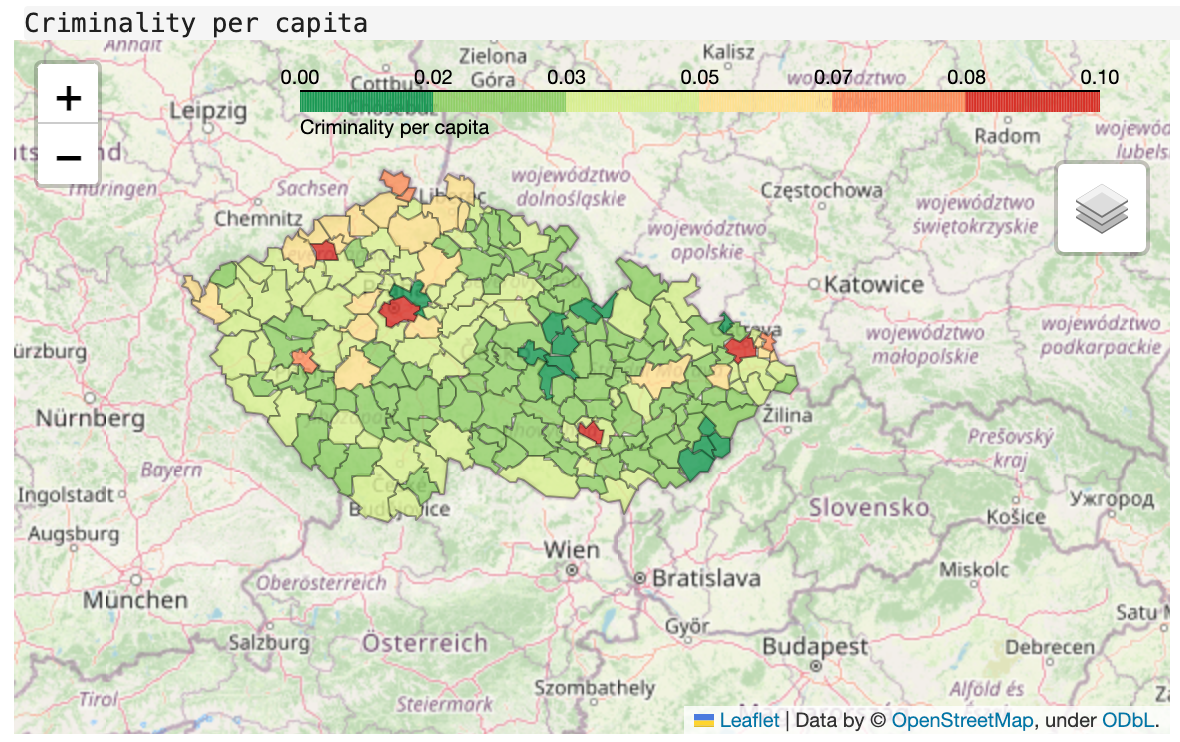
\includegraphics[width=.8\textwidth]{Criminality_per_capita.png}
\end{center}
\paragraph{\normalfont{Here we can see that except the 3. and 5. position we see cities that are not really often in the worst 5 in all of the other measures. Thus we can see quite a strong ommited variable bias which is not captured in the independent varibles.}}
\begin{center}
    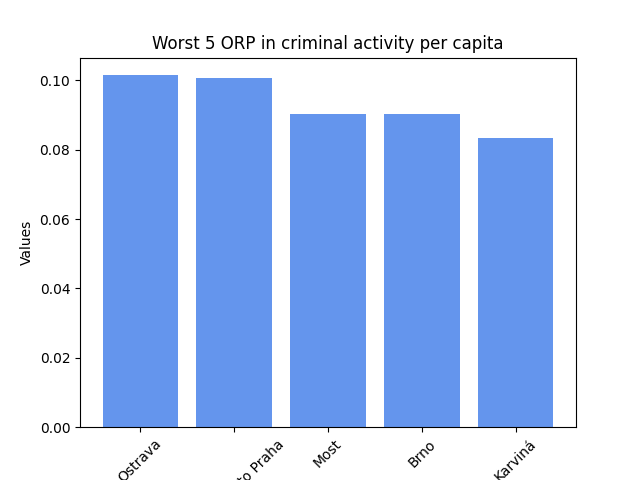
\includegraphics[width=.8\textwidth]{Worst 5 ORP in criminal activity per capita.png}
\end{center}

\paragraph{\normalfont{Secondly, we plotted already mentioned socio-economic indicators and their geographical structure across the whole Czech Republic. For each of them we again show the worst regions where the lawmakers should focus in the future.}}
\begin{center}
    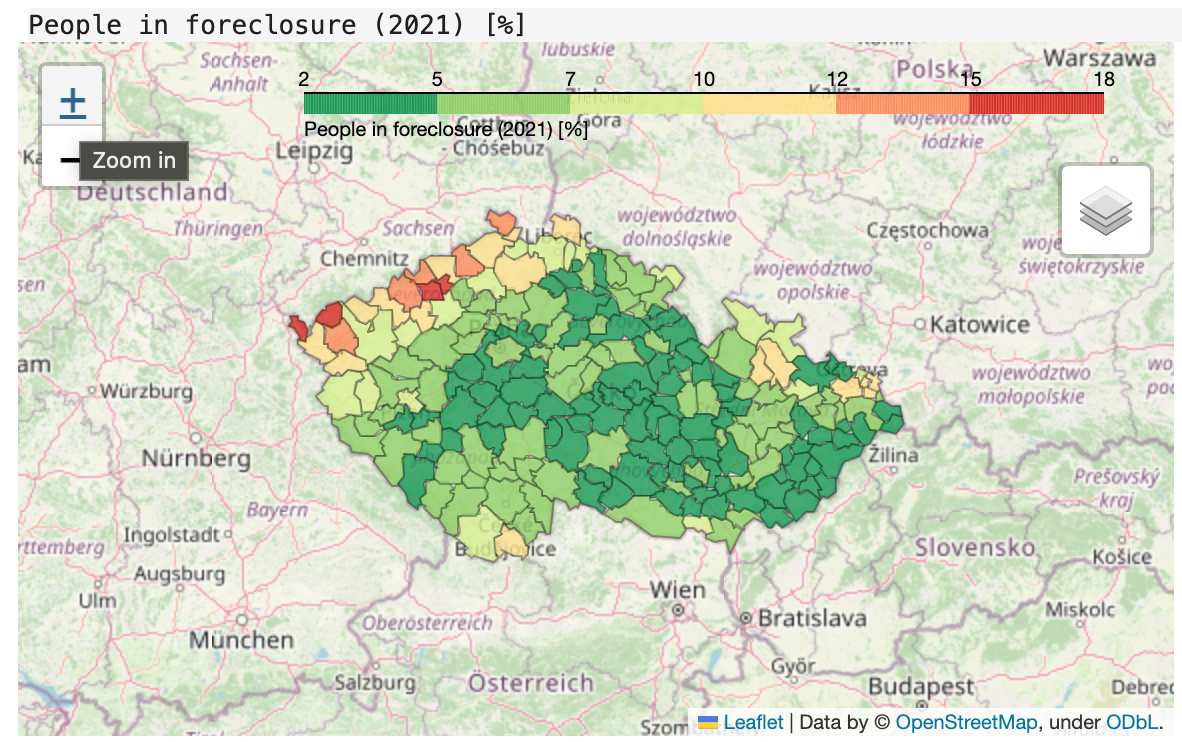
\includegraphics[width=.8\textwidth]{people_in_foreclosure.png}
    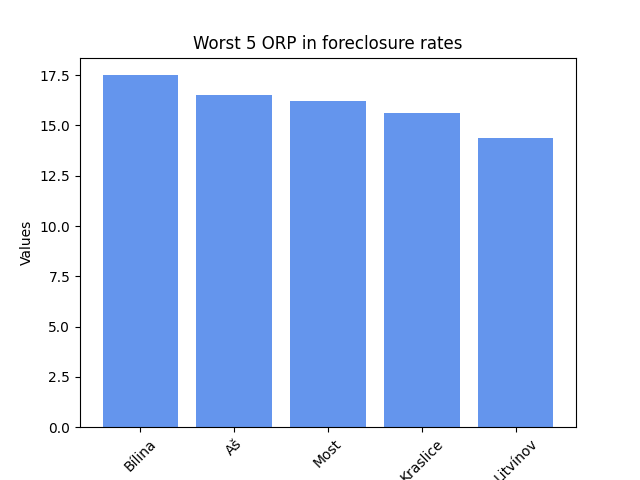
\includegraphics[width=.8\textwidth]{Worst 5 ORP in foreclosure rates.png}
    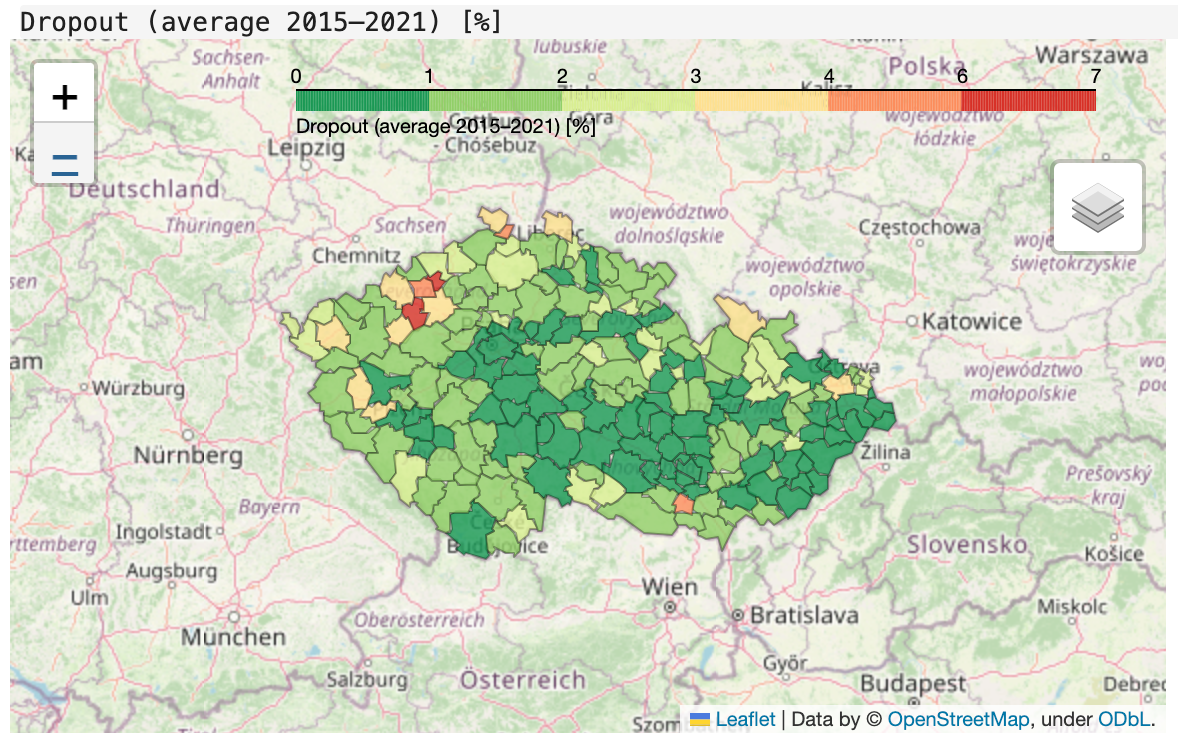
\includegraphics[width=.8\textwidth]{dropout.png}
    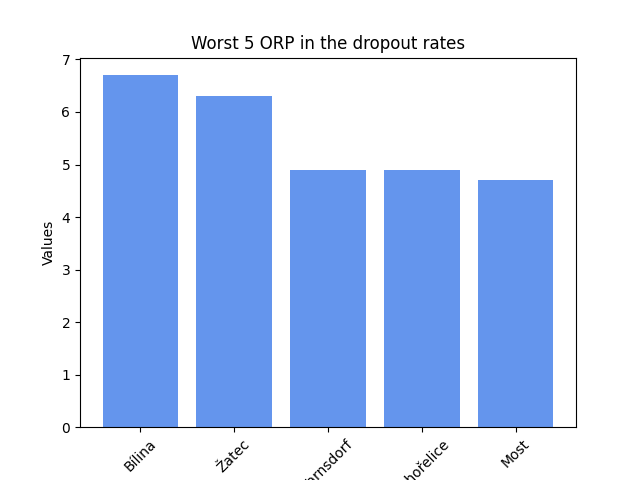
\includegraphics[width=.8\textwidth]{Worst 5 ORP in the dropout rates.png}
    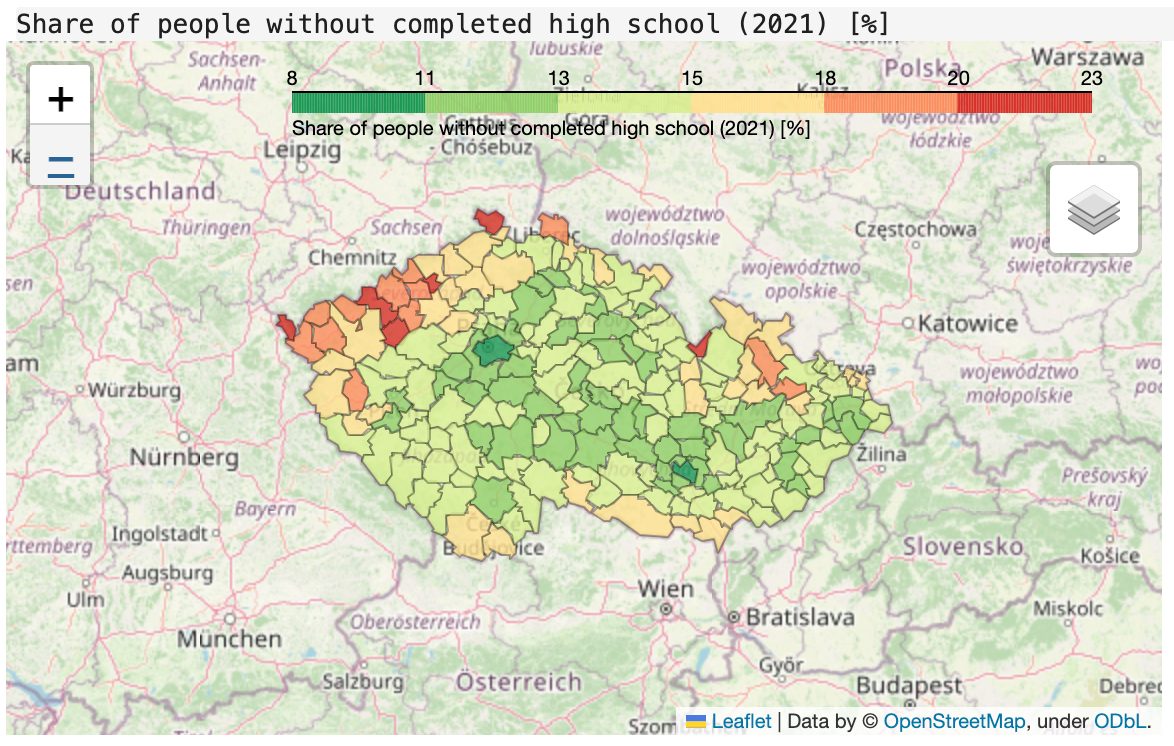
\includegraphics[width=.8\textwidth]{without_high_school.png}
    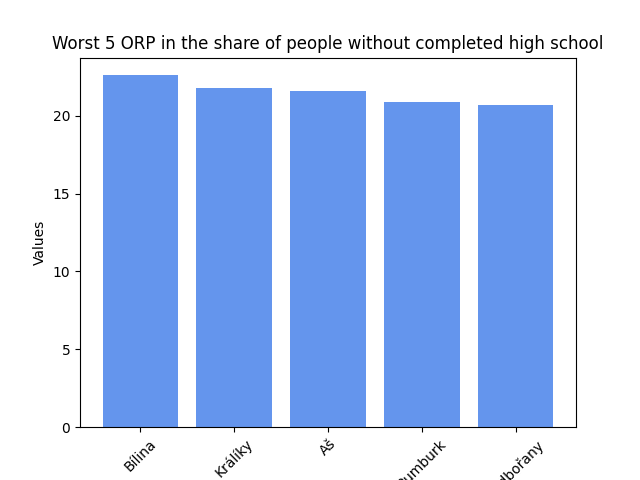
\includegraphics[width=.8\textwidth]{Worst 5 ORP in the share of people without completed high school.png}
    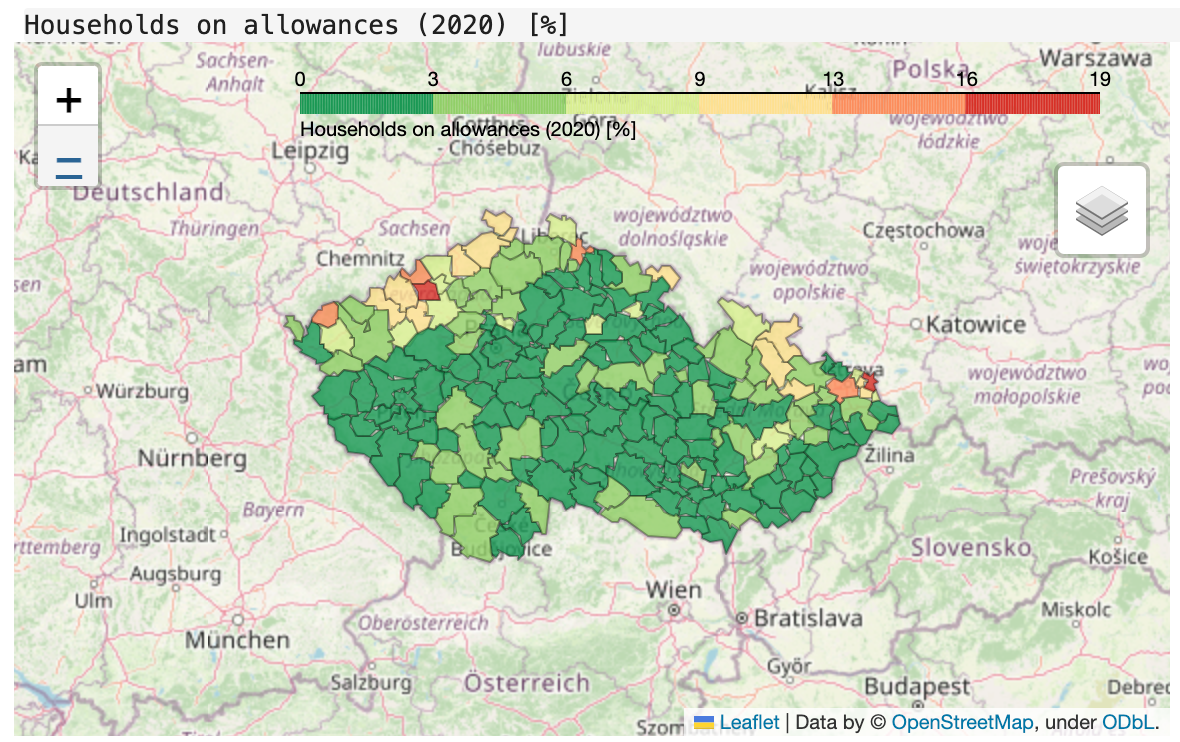
\includegraphics[width=.8\textwidth]{allowances.png}
    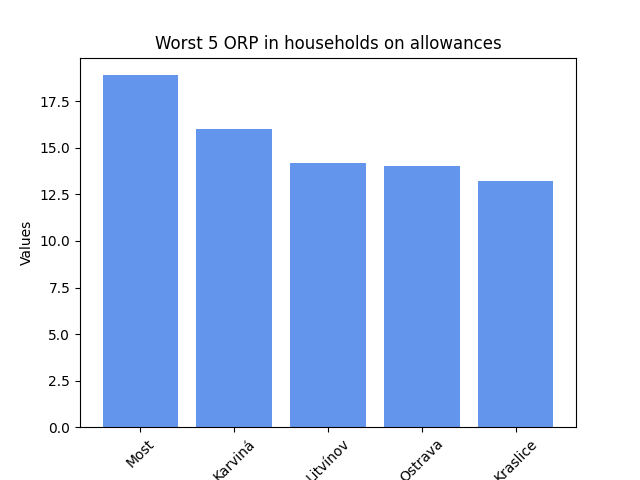
\includegraphics[width=.8\textwidth]{Worst 5 ORP in households on allowances.png}
\end{center}

\paragraph{\normalfont{Then, according to the procedure mentioned in "Code Overview" and which you can find on GitHub (https://github.com/Tomas-Barhon/Python-project), we used the data to create \textbf{Criminality risk index} that finally shows which ORPs are according to our analysis the most keen to economic crime acts. As you can see, the red area around Ústí nad Labem close to the German borders indicates a high rate of crimes. Ostrava and near cities follow as the second most criminal area in the Czech Republic. On the opposite, Prague or Brno, for example, came out as a safe space when we compare the findings to the initial maps. For all data we took for the criminality index, we took the number of inhabitants in the areas into consideration and count it per capita.}}
\begin{center}
    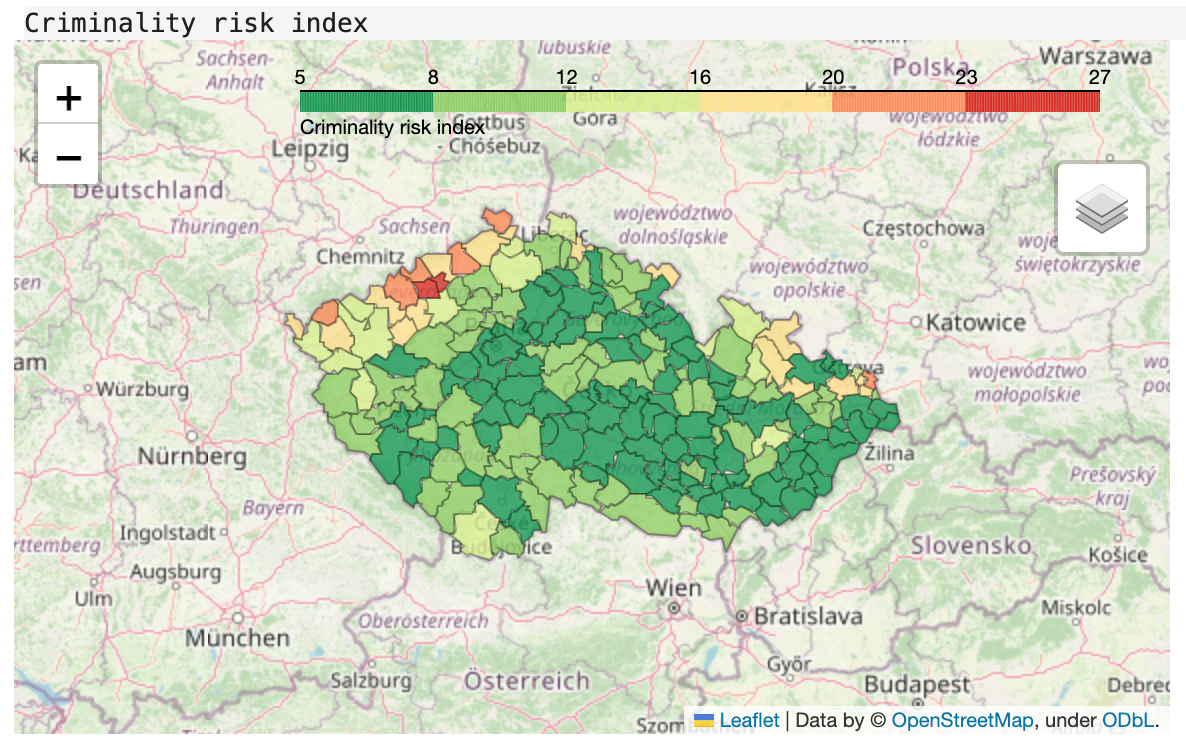
\includegraphics[width=.8\textwidth]{risk_index.png}
    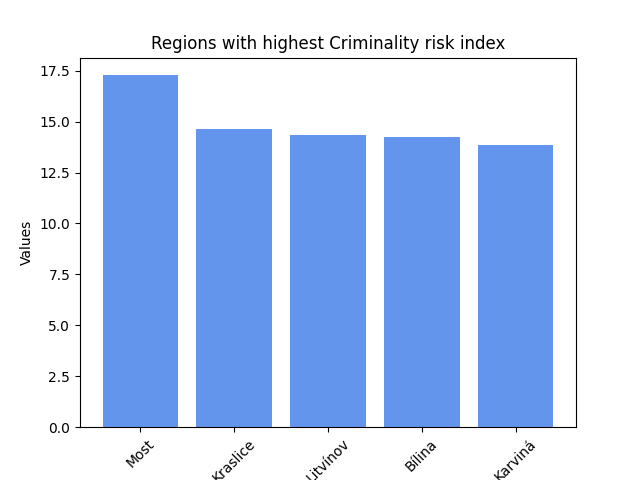
\includegraphics[width=.8\textwidth]{Regions with highest Criminality risk index.png}
\end{center}

\paragraph{\normalfont{As a further analysis, we plot individual indicators on the correlation graph to really see how much these indicators correlate with the number of criminal activities per capita. You can see the graphs below.}}
\begin{center}
    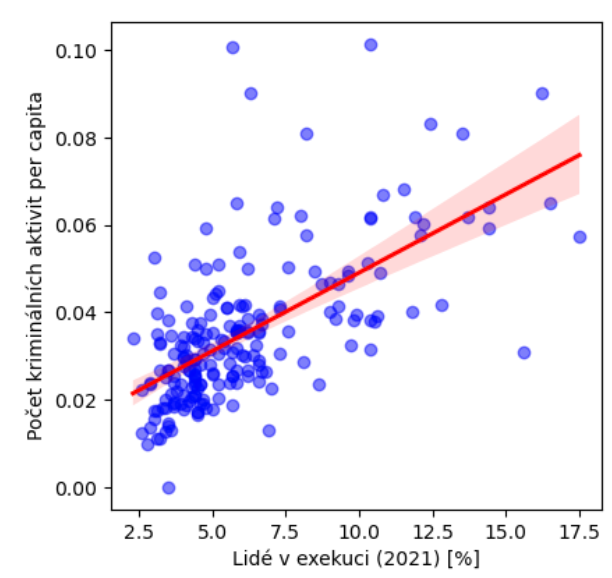
\includegraphics[width=.8\textwidth]{corr1.png}
    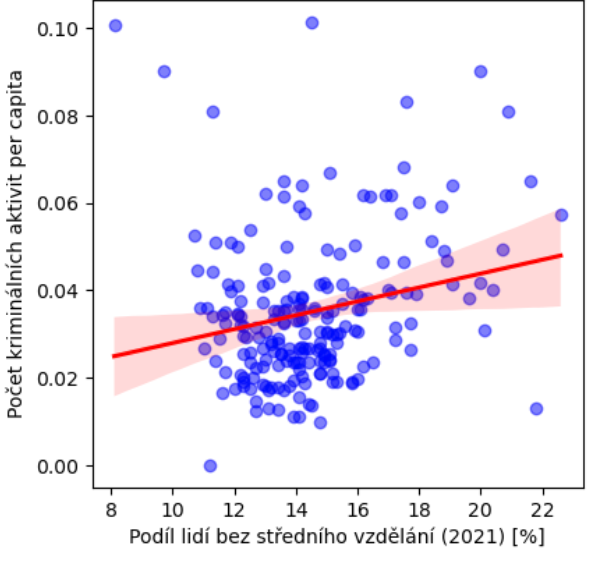
\includegraphics[width=.8\textwidth]{corr2.png}
    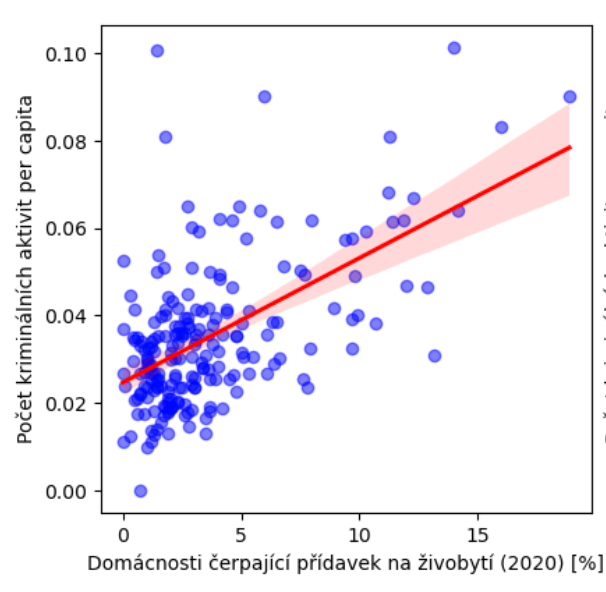
\includegraphics[width=.8\textwidth]{corr3.png}
    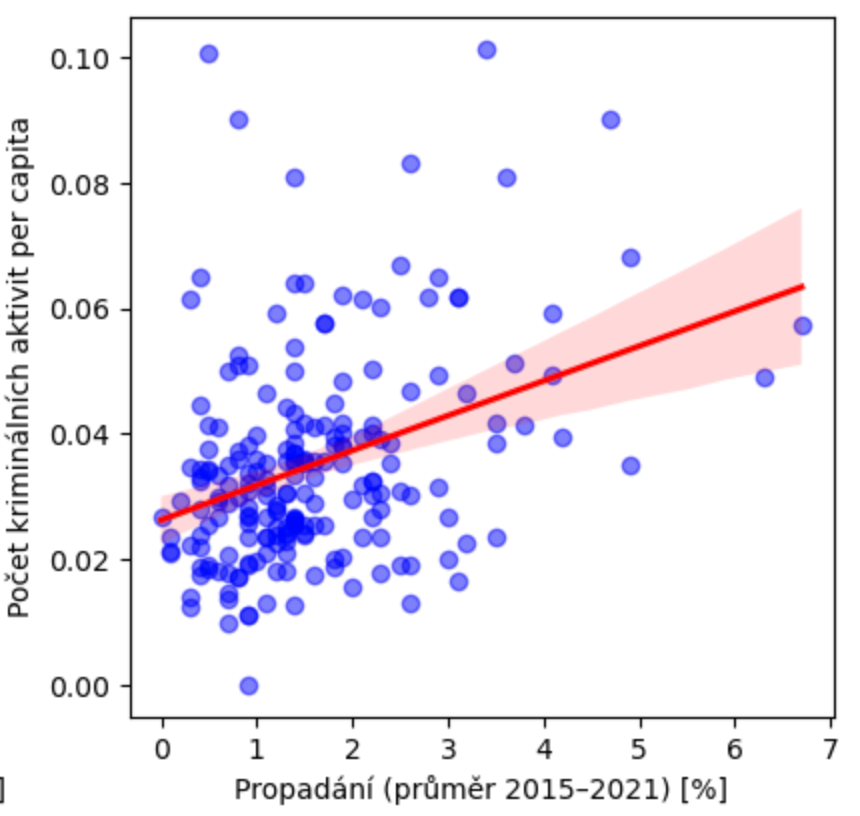
\includegraphics[width=.8\textwidth]{corr4.png}
\end{center}

\paragraph{\normalfont{As you can see, the most correlated with the number of criminal activities per capita is "The percentage of people with foreclosure" (0.63) and "The percentage of households receiving social benefits" (0.57) which are almost of the same correlation. On the other hand, the least correlated is "The percentage of people without completed high school education" (0.22) which does not influence the number of criminality in the regions as much - it also has the biggest deviation of the all mentioned indicators (which makes sense). Exact correlation numbers are visualized below on the correlation scale.}}
\begin{center}
    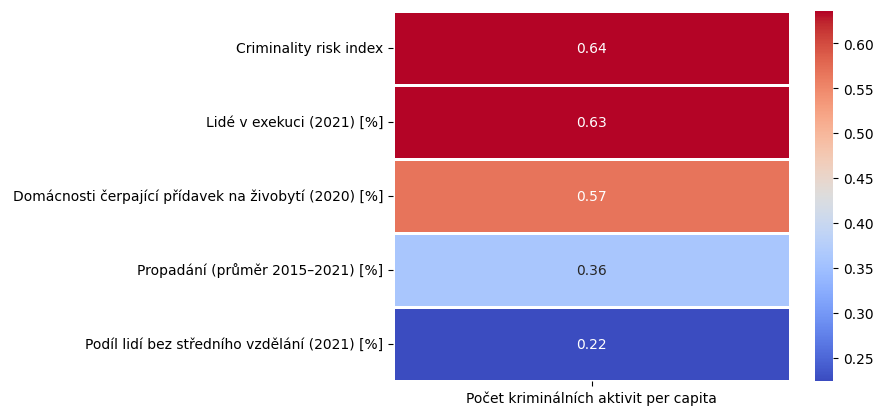
\includegraphics[width=.8\textwidth]{heat_map.png}
\end{center}

\section{References}
\paragraph{\normalfont{The data used in this project, that we acquired from PAQ research, were obtained from various sources including the Czech Statistical Office, the Agency for Social Inclusion, the Ministry of Labour and Social Affairs, the Chamber of Executors of the Czech Republic, and the Czech Household Panel Study.}}

\paragraph{\normalfont{The records of crime acts are exclusively from the Police of the Czech Republic which as the only one has the resources for it. }}

\begin{enumerate}
\item https://www.datapaq.cz/
\item PAQ data endpoints:
\item Domácnosti čerpající přídavek na živobytí (2020) po ORP - Agentura pro sociální začleňování, MPSV
\item Podíl lidí bez středního vzdělání - ČSÚ, SLDB 2021
\item Propadání (2015-2021)- ČŠI
\item Lidé v exekuci (2021)- Exekutorská komora ČR, ČSÚ, Czech Household Panel Study
\item https://kriminalita.policie.cz/
\item https://www.czso.cz/csu/xs/obyvatelstvo-xs Czech Statistical office - the data on the population in each ORP as the data was in quite a messy Excel file, we had to transform it manually and the new table is now to your disposal in our repository (app/počet\_obyvatel\_ORP.xlsx) and can be used in other projects with similar nature. It makes it easier to share the project with others.
\end{enumerate}

\bibliographystyle{apa}
\bibliography{bibliography.bib}	

\end{document}